
\section{Estimating network parameters}
\label{sec:nw_par_est}


To use the \kf{} in any meaningful way, we first need to estimate the system noise, $\NWnoise_\ell$, and the between-vehicle variance, $\NWvar_{\ell}^2$. To estimate values for these parameters, we fit the same model from \cref{sec:nw_model} to the historical data shown in \cref{fig:tt_figure} using \gls{mcmc} sampling methods as implemented by \prog{JAGS} \citep{JAGS}.


The first step in the modelling process fits the following hierarchical model:
\begin{equation}
\label{eq:nw_model_simple}
\left\{
\begin{split}
\Vttobs_{\ellc}^m &\sim \Normal{\Vtt_{\ellc}^m}{(\Vtterr_{\ellc}^m)^2} &
\NWstate_{\ell,0} &\sim \Uniform{0}{\MaxSpeed_\ell} \nonumber \\
\Vtt_{\ellc}^m &\sim \TNormal{\NWstate_{\ellc}}{\NWvar_{\ell}^2}{0}{\MaxSpeed_\ell} &
\NWvar_\ell &\sim \GammaD{0.01}{0.01} \\
\NWstate_{\ellc} &\sim \TNormal{\NWstate_{\ell-1,c}}{(\NWtdiff_c \NWnoise_{\ell})^2}{0}{\MaxSpeed_\ell} &
\NWnoise &\sim \GammaD{0.01}{0.01} \nonumber
\end{split}
\right. .
\end{equation}
The observation error, as in the previous section, is assumed to be constant for all observations, $\Vtterr_{\ellc}^m = 0.8$~\gls{mps} (which is about 10~km/h). The model implementation was performed from \Rstats{} using the \pkg{rjags} package \citep{rjags}. The model output was processed using the \pkg{tidybayes} package \citep{tidybayes} and graphed using \pkg{ggplot2} \citep{ggplot2}. The \pkg{coda} package was used to assess the model's convergence results \citep{coda}.


\subsection{Simulated data}
\label{nw_par_est_sim}

\begin{knitrout}\small
\definecolor{shadecolor}{rgb}{0.969, 0.969, 0.969}\color{fgcolor}\begin{figure}

{\centering 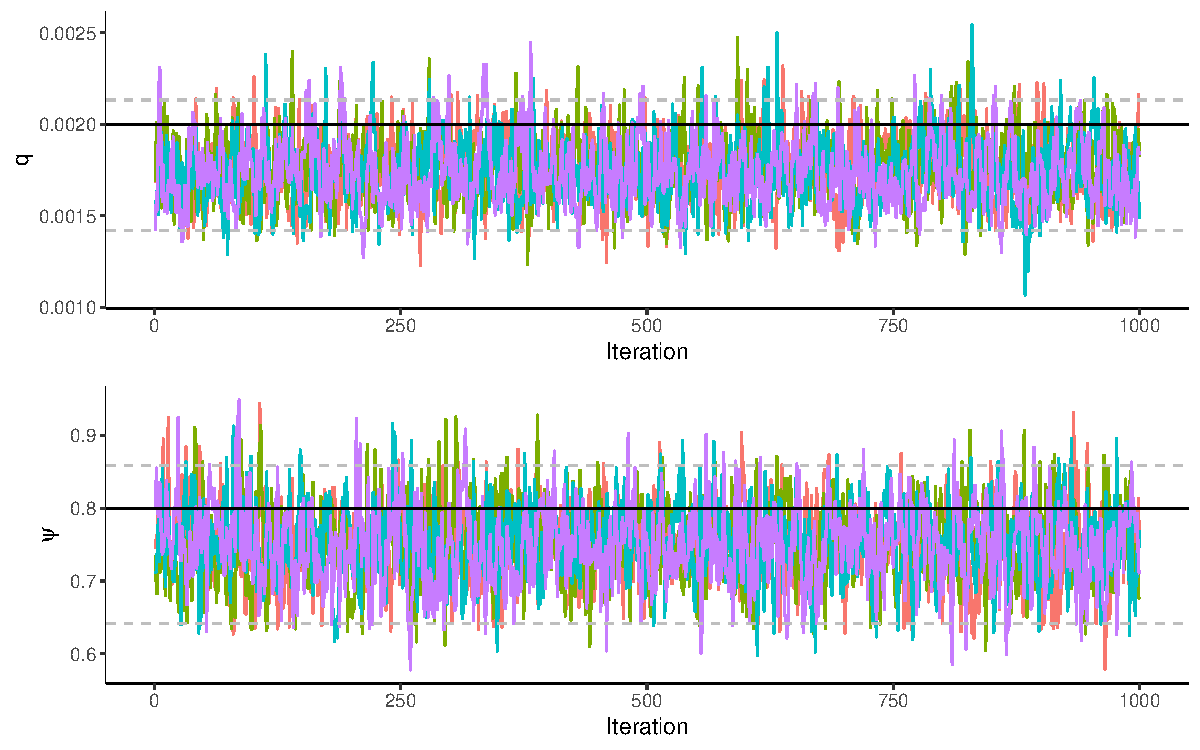
\includegraphics[width=0.8\textwidth]{figure/nw_model_sim_results-1} 

}

\caption[Traceplots of model parameters for the simulated data]{Traceplots of model parameters for the simulated data. Each of the four chains are coloured separately. Dashed grey lines show the 95\% posterior credible interval and the solid lines represent the true values or each parameter.}\label{fig:nw_model_sim_results}
\end{figure}


\end{knitrout}


To assess the model, we start by fitting it to the simulated data (\cref{fig:nw_sim_data}), for which we know the values of $\NWnoise_\ell$ and $\NWvar_\ell$. Trace plots of the model parameters shown in \cref{fig:nw_model_sim_results}, with the true values overlaid with a dashed line, show that the chains mixed well. \Cref{tab:nw_model_sim_smry} gives a summary of the simulation values and their posterior estimates, along with convergence statistics. The 95\% credible intervals for the two parameters contain the true values, so there is nothing to suggest the model is inadequate for modelling the simulated data and estimating the network parameters.


\begin{table}

\caption{\label{tab:nw_model_sim_smry}Simulation MCMC results. The multivariate $\hat R$, including for all of the $\NWstate$ parameters, was 1.04, indicating that convergence had been achieved after 15,000 iterations.}
\centering
\begin{tabular}[b]{llllllr}
\toprule
Parameter & True Value & Mean & 2.5\% & 50\% & 97.5\% & $\hat R$\\
\midrule
$\NWnoise_\ell$ & 0.002 & 0.0017 & 0.0014 & 0.0017 & 0.0021 & 1.001\\
$\NWvar_\ell$ & 0.8 & 0.75 & 0.64 & 0.75 & 0.86 & 1.001\\
\bottomrule
\end{tabular}
\end{table}





\subsection{Real data}
\label{nw_par_est_real}



Having shown that the \prog{JAGS} model is a valid way of estimating the network parameters $\NWnoise_\ell$ and $\NWvar_\ell$, we model the real travel time data from \cref{fig:tt_figure}. Trace plots of the network parameters, as shown in \cref{fig:nw_model_n1_view}, show again that the chains mixed well, which is reaffirmed by the convergence results in \cref{tab:nw_model_fit_smry}. Not shown here are the summaries of the $\NWstate$'s (there are 187 of them); however, the Gelman diagnostic $\hat R$ was less than 1.03 for all of them, indicating they reached convergence.

\begin{knitrout}\small
\definecolor{shadecolor}{rgb}{0.969, 0.969, 0.969}\color{fgcolor}\begin{figure}

{\centering 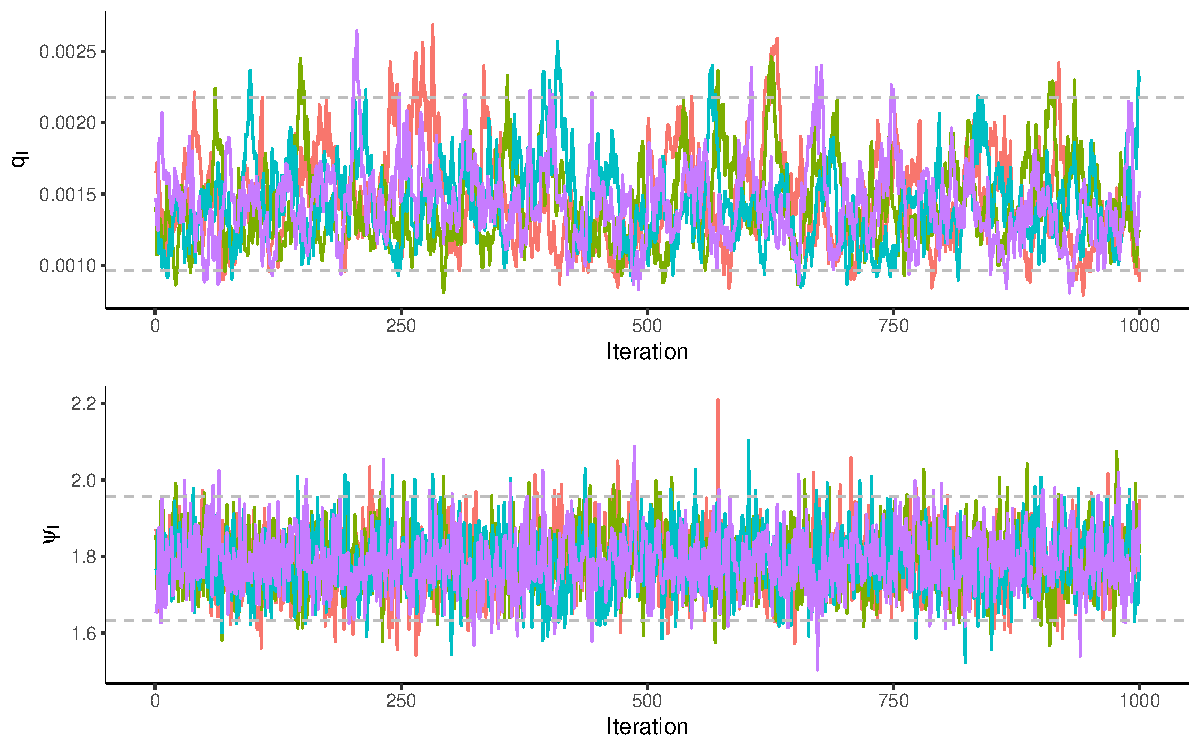
\includegraphics[width=0.8\linewidth]{figure/nw_model_n1_view-1} 

}

\caption[Traceplots of model parameters fitted to the segment data]{Traceplots of model parameters $\NWnoise$ and $\NWvar$ fitted to the segment data. Each of the four chains are coloured separately. The 95\% posterior credible region is denoted by dashed grey lines.}\label{fig:nw_model_n1_view}
\end{figure}


\end{knitrout}

\begin{table}

\caption{\label{tab:nw_model_fit_smry}MCMC results for the average segment speeds. The multivariate $\hat R$, including for all of the $\NWstate$ parameters, was 1.08, indicating that convergence had been achieved after 15,000 iterations.}
\centering
\begin{tabular}[b]{lllllr}
\toprule
Parameter & Mean & 2.5\% & 50\% & 97.5\% & $\hat R$\\
\midrule
$\NWnoise_\ell$ & 0.0015 & 0.001 & 0.0015 & 0.0022 & 1.013\\
$\NWvar_\ell$ & 1.94 & 1.8 & 1.94 & 2.1 & 1.002\\
\bottomrule
\end{tabular}
\end{table}



To assess the adequacy of these parameters, we fit the \kf{} to the same data\footnote{In the next section we use two weeks of data, one for each of testing and training.} to see how well the mean and predictive distributions fit the data. The estimates of $\NWstate_{\ell,1:c}$, along with associated uncertainties, are shown in \cref{fig:nw_model_n1_kf1}, where we see that the mean approximately follows the center of the data. The predictive vehicle speed distribution, which accounts for both $\NWstatevar_{\ell,1:c}$ and vehicle variation, $\NWvar_{\ell}^2$, is shown in \cref{fig:nw_model_n1_kf2}, and shows most of the points contained within the 95\% posterior predictive region.


\begin{knitrout}\small
\definecolor{shadecolor}{rgb}{0.969, 0.969, 0.969}\color{fgcolor}\begin{figure}

{\centering \subfloat[Estimated mean speed, showing state estimates along with the 95\% credible region.\label{fig:nw_model_n1_kf1}]{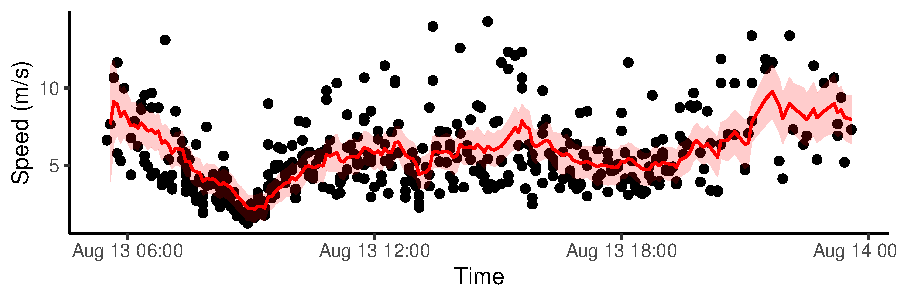
\includegraphics[width=.8\textwidth]{figure/nw_model_n1_kf-1} }\\
\subfloat[Predictive distribution of vehicle speeds, which includes between-vehicle variability.\label{fig:nw_model_n1_kf2}]{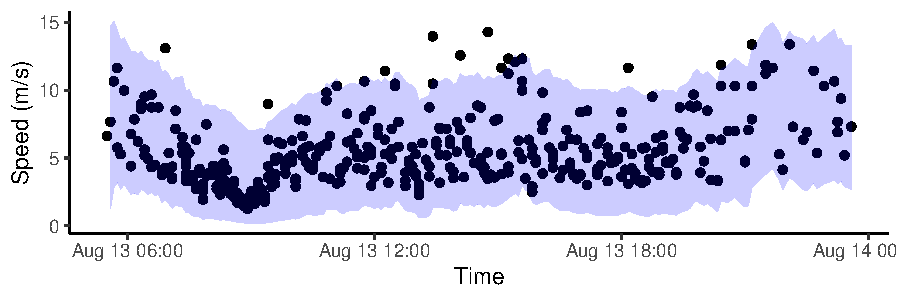
\includegraphics[width=.8\textwidth]{figure/nw_model_n1_kf-2} }\\

}

\caption[Results of fitting a \kf{} to the segment data with parameters estimated using the hierarchical model]{Results of fitting a \kf{} to the segment data with parameters estimated using the hierarchical model.}\label{fig:nw_model_n1_kf}
\end{figure}


\end{knitrout}



Finally, the timing comparison is displayed in \cref{tab:nw_model_n1_timecomp}. The hierarchical model fit using \prog{JAGS} took about 2200 times as long as the \kf{} implementation. So, even if we reduced the number of chains, the number of iterations, and tried to speed up the \prog{JAGS} model, the \kf{} would still be significantly faster.


\begin{table}

\caption{\label{tab:nw_model_n1_timecomp}Timing results (seconds).}
\centering
\begin{tabular}[b]{lrrr}
\toprule
  & User & System & Total\\
\midrule
JAGS & 123.264 & 0.004 & 123.273\\
Kalman filter & 0.044 & 0.000 & 0.046\\
\bottomrule
\end{tabular}
\end{table}




\subsection{Hierarchical model over multiple road segments}
\label{sec:nw_par_est_multiple}



To assess how effective our approach is for estimating $\NWvar_\ell$ and $\NWnoise_\ell$, we selected five other road segments around Auckland. However, instead of fitting the same model independently to each segment,  we use a hierarchical Bayesian model on the parameters, since it seems reasonable that, while they will not be the same for all segments, there will be an underlying population distribution. This allows us to obtain estimates of the parameter values without explicitly needing to model every road (of which there are 8,151).


The hierarchical model used to estimate the network parameters is:
\begin{equation}
\label{eq:tt_hist_hier}
\left\{
\begin{split}
\Vttobs_{\ellc}^m &\sim \Normal{\Vtt_{\ellc}^m}{\left(\Vtterr_{\ellc}^m\right)^2} &
\NWstate_{\ell0} &\sim \Normal{0}{10^2} \\
\Vtt_{\ellc}^m &\sim \TNormal{\NWstate_{\ellc}}{\NWvar_{\ell}^2}{0}{\MaxSpeed_\ell} &
\mu_\psi &\sim \Normal{0}{10^2} \\
\NWstate_{\ellc} &\sim \TNormal{\NWstate_{\ellc-1}}{(\NWtdiff_c \NWnoise_{\ell})^2}{0}{\MaxSpeed_\ell} &
\sigma_\psi &\sim \GammaD{0.001}{0.001} \\
\log\left(\NWvar_{\ell}\right) &\sim \Normal{\mu_\psi}{\sigma_\psi^2} &
q &\sim \GammaD{0.001}{0.001}
\end{split}
\right. .
\end{equation}
We initially attempted to fit a hierarchical segment noise parameter $\NWnoise_{\ell}$ with hyperparameters, but the values were all approximately equal for all segments and convergence was very slow (100,000's of iterations). Instead, we opted for a single common system noise parameter across all segments. The speed data for six segments on two consecutive Tuesdays is shown in \cref{fig:nw_model_n2_segplots}, with the locations of the roads displayed in \cref{fig:nw_seg_maps}.

\begin{knitrout}\small
\definecolor{shadecolor}{rgb}{0.969, 0.969, 0.969}\color{fgcolor}\begin{figure}

{\centering 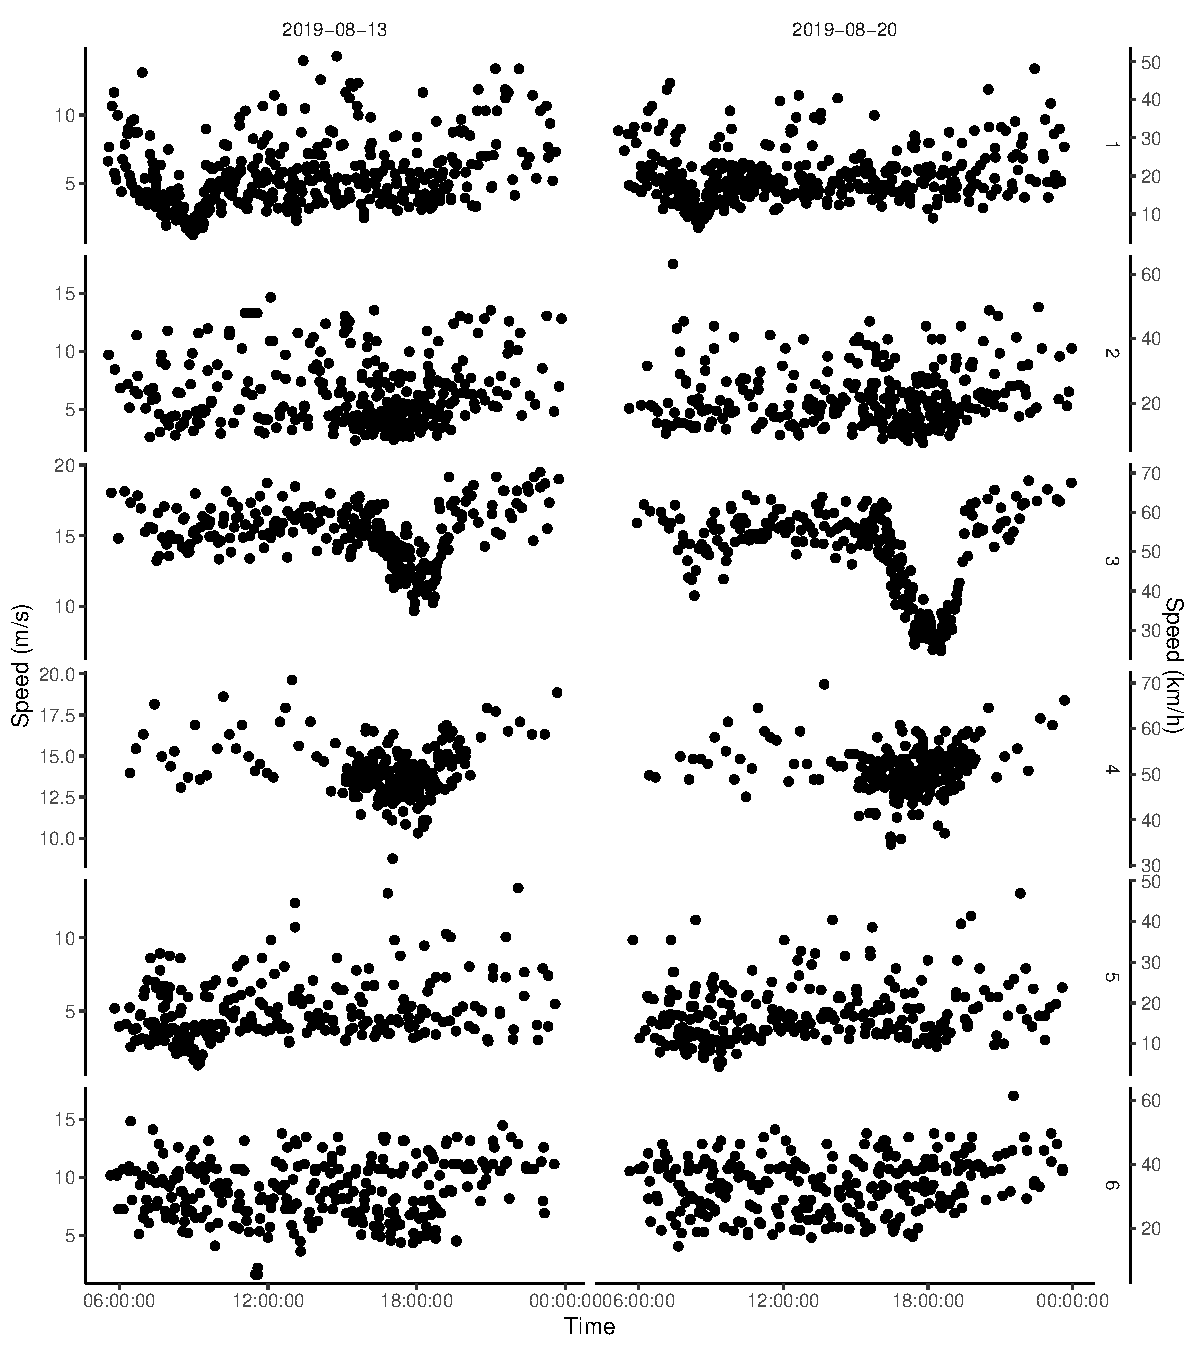
\includegraphics[width=\textwidth]{figure/nw_model_n2_segplots-1} 

}

\caption[Observed average bus speeds along six road segments on two consecutive Tuesdays]{Observed average bus speeds along six road segments on two consecutive Tuesdays.}\label{fig:nw_model_n2_segplots}
\end{figure}


\end{knitrout}

\begin{knitrout}\small
\definecolor{shadecolor}{rgb}{0.969, 0.969, 0.969}\color{fgcolor}\begin{figure}

{\centering 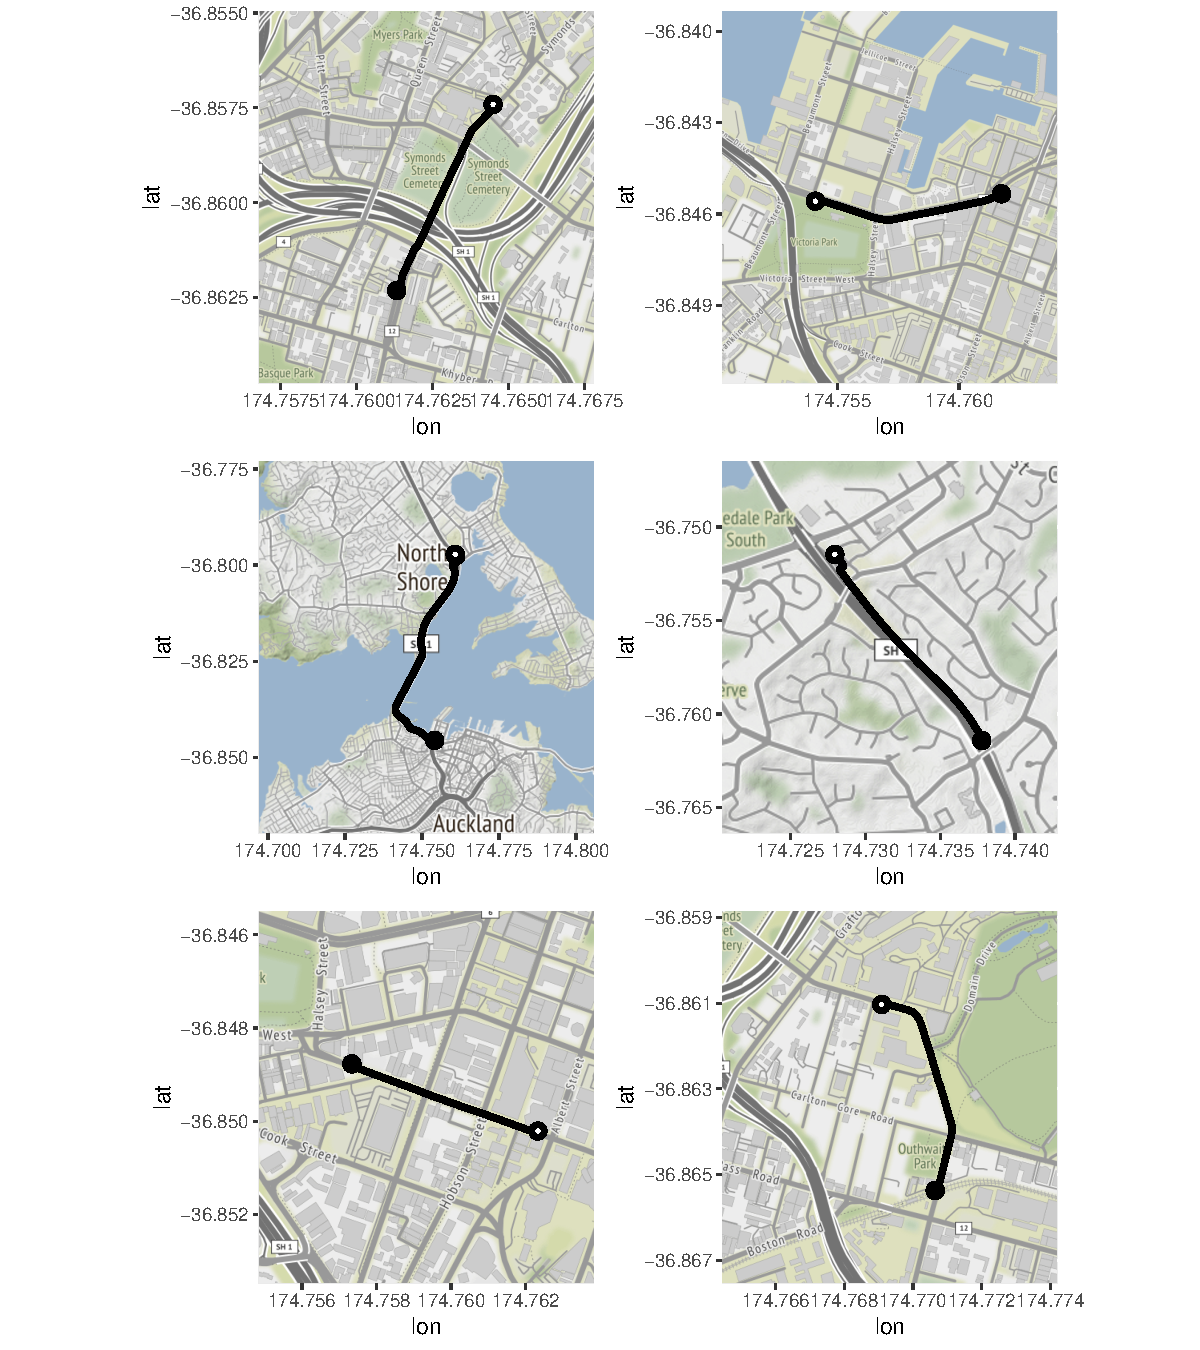
\includegraphics[width=\textwidth]{figure/nw_seg_maps-1} 

}

\caption[Segment locations, drawn using the \pkg{ggmap} package \citep{ggmap}]{Segment locations, drawn using the \pkg{ggmap} package \citep{ggmap}. Segments begin at the solid point and terminate at the open point.}\label{fig:nw_seg_maps}
\end{figure}


\end{knitrout}




\begin{knitrout}\small
\definecolor{shadecolor}{rgb}{0.969, 0.969, 0.969}\color{fgcolor}\begin{figure}

{\centering 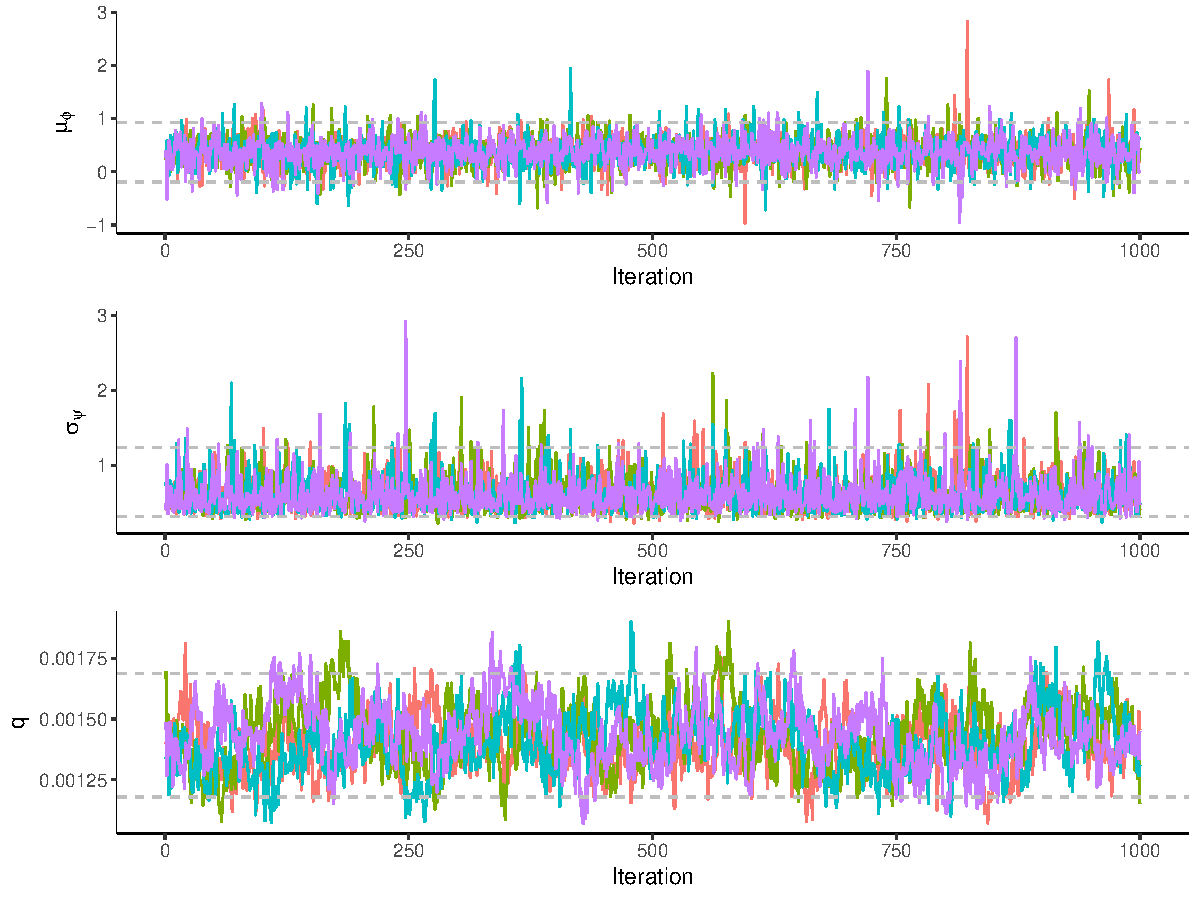
\includegraphics[width=\textwidth]{figure/nw_model_n2_diag-1} 

}

\caption[Traceplots of top-level network parameters estimated by the hierarhical model]{Traceplots of top-level network parameters estimated by the hierarhical model. The four chains are coloured individually, and 95\% credible interval indicated by dashed gray lines.}\label{fig:nw_model_n2_diag}
\end{figure}


\end{knitrout}


\begin{table}

\caption{\label{tab:nw_model_n2_smry}MCMC results for the top-level parameters for the hierarchical segment model. The multivariate $\hat R$, including for all of the $\NWstate$ parameters, was 2.03.}
\centering
\begin{tabular}[b]{lllllr}
\toprule
Parameter & Mean & 2.5\% & 50\% & 97.5\% & $\hat R$\\
\midrule
$\mu_\psi$ & 0.383 & -0.191 & 0.389 & 0.926 & 1.00\\
$\sigma_\psi$ & 0.608 & 0.315 & 0.549 & 1.24 & 1.00\\
$q$ & 0.0014 & 0.0012 & 0.0014 & 0.0017 & 1.02\\
\bottomrule
\end{tabular}
\end{table}




The model was fit using \prog{JAGS} to the first day of data for the six segments, while the second was reserved for testing the validity of the estimated parameters. Each of the four chains was run with a 100,000~iteration burn-in phase, followed by 50,000 iterations with a thinning interval of 50. Trace plots of the top-level parameters are displayed in \cref{fig:nw_model_n2_diag}, which demonstrates good mixing of the chains. \Cref{tab:nw_model_n2_smry} shows the posterior mean and quantiles for these parameters, along with their Gelman convergence diagnostics.


Trace plots for the segment-specific variance parameters are shown in \cref{fig:nw_model_n2_diag_2}, and also demonstrate good mixing. The Gelman convergence diagnostic is again very close to unity, indicating that running the chain for longer would not decrease the posterior variance by much.



\begin{knitrout}\small
\definecolor{shadecolor}{rgb}{0.969, 0.969, 0.969}\color{fgcolor}\begin{figure}

{\centering 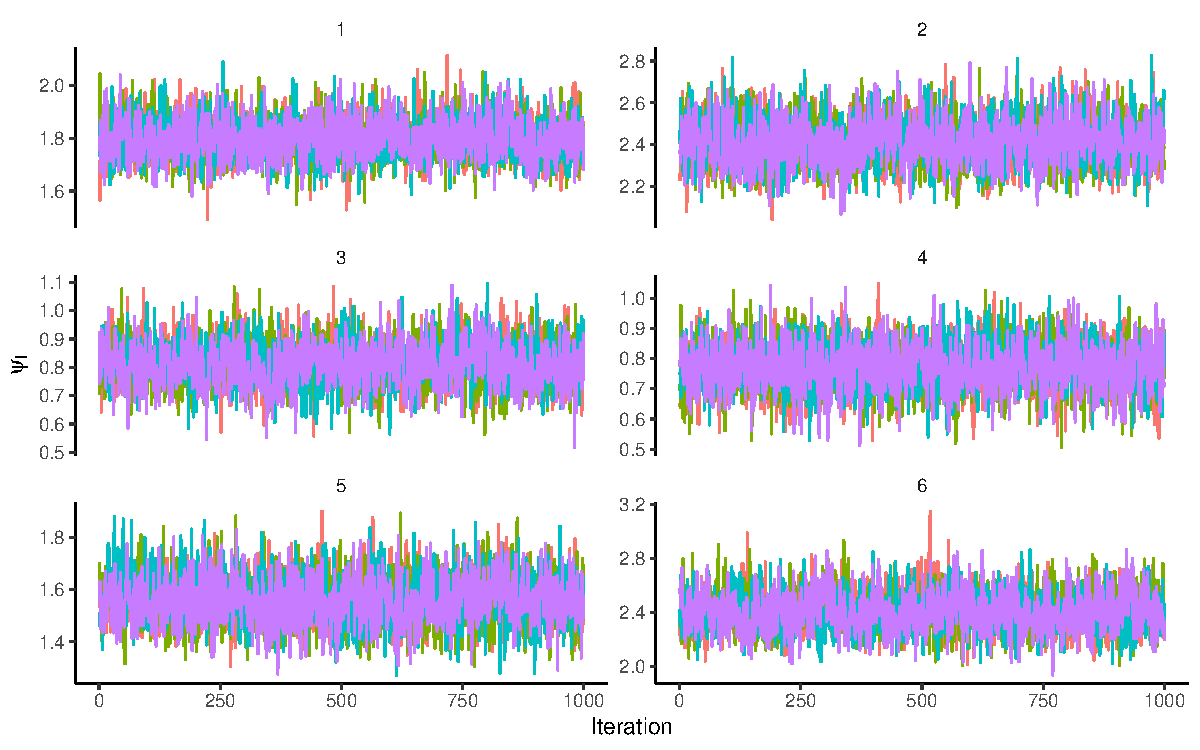
\includegraphics[width=\textwidth]{figure/nw_model_n2_diag_2-1} 

}

\caption[Traceplots of between-vehicle variance parameters, $\NWvar_\ell$, for each segment]{Traceplots of between-vehicle variance parameters, $\NWvar_\ell$, for each segment. The four chains are coloured individually.}\label{fig:nw_model_n2_diag_2}
\end{figure}


\end{knitrout}


The \kf{} was fit to each segment using the posterior mean of $\NWvar_\ell$ and the population parameters. \Cref{fig:nw_model_n2_kf} shows the original data superimposed with a posterior sample of $\NWstate$'s, along with the next week's data with results from the \kf{}, including the 95\% credible region for the mean travel time and the 95\% posterior predictive region for individual vehicle travel times.







\begin{knitrout}\small
\definecolor{shadecolor}{rgb}{0.969, 0.969, 0.969}\color{fgcolor}\begin{figure}
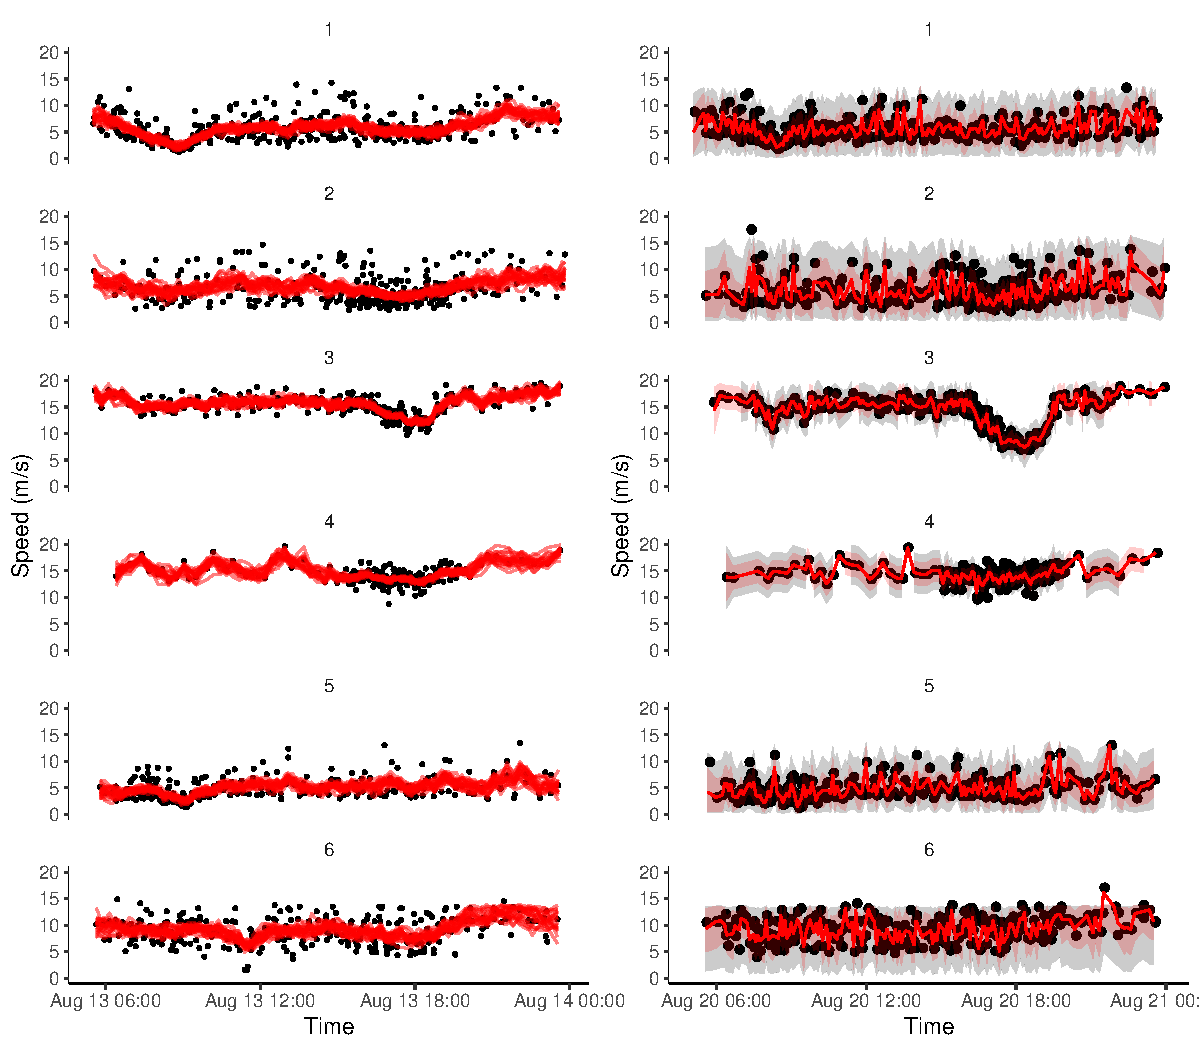
\includegraphics[width=\textwidth]{figure/nw_model_n2_kf-1} \caption[Results for the hierarchical approach to modelling road speed]{Results for the hierarchical approach to modelling road speed. Left: the training data with a sample of posterior fits for \prog{JAGS}. Right: the test data with the Kalman filter estimation results, showing the speed estimate (red line), its uncertainty (shared in red), and the posterior predictive region for vehicle speeds (shaded in grey).}\label{fig:nw_model_n2_kf}
\end{figure}


\end{knitrout}

The results show that the $\NWstate$ values estimated with \prog{JAGS} nicely fit the data, including peak congestion, as do the \kf{} estimates. The posterior predictive region covers most of the observations for all the segments.
